\subsection{Gaussian Processes}
\label{sec:gps}

A Gaussian process is a non-parametric ML method.
It describes a collection of random variables, every finite collection of which follows a multivariate Gaussian distribution.

Training a GP involves taking as input 

Since the GP specifies a prior over functions, it also has a notion of its likelihood on its input training points.

\begin{equation}
K(x,x') = \exp \left( - \frac{(x - x')^2}{2 l^2} \right)
\end{equation}

\hl{Say smth about setting the kernel using the points in the interior and then evaluate it on points in the exterior}

We use a Gaussian Process to fit $p (m_{h1}, m_{h2})$.


The input to the GP is a 2d histogram of the massplane (as visualized in \Fig{\ref{massplane_obs_18}}. The massplane is the bounding box centered on the SR center and the length (or size) of the box edge is 90~GeV, using 25 bins for both the $m_{H1}$ and $m_{H2}$ axes. We specify each bin of this histogram by its center and model the number of events in the bin. Bins that have any overlap with the SR are not included in the training process. We fit the GP using scikit-learn \cite{scikit-learn}.
The input training points are the centers of the bins, and the observed data that we predict are 

\begin{equation}
K \left(
\begin{bmatrix}
m_{H1} \\
m_{H2}
\end{bmatrix},
\begin{bmatrix}
m_{H1}' \\
m_{H2}'
\end{bmatrix}
\right)
 = \exp\left( - \frac{\left(m_{H1} - m_{H1}' \right)^2}{2 l_1^2} -  \frac{\left(m_{H2} - m_{H2}' \right)^2}{2 l_2^2}  \right)
\end{equation}

To account for the differences in the triggers, we fit a separate GP for each year (2016, 2017, and 2018), and the GP fit and predicted error for 2018 are shown in \Fig{\ref{massplane_pred_18}} and \ref{massplane_prederr_18}, respectively. By eye you can already see that the predicted massplane follows the characteristic kinematics of the input massplane, while also providing a smooth interpolation into the SR. The GP also has a notion of its uncertainty, as you can see that the error increases slightly as we go into the SR. 

\def\valreg{4b}
\def\vallabel{4b signal}%reversed $\Delta \eta_{HH}$}
\def\figpath{figures/flows/\valreg/}

\begin{figure}[ht]
    \centering
    \subfloat[observed data]{ 
    	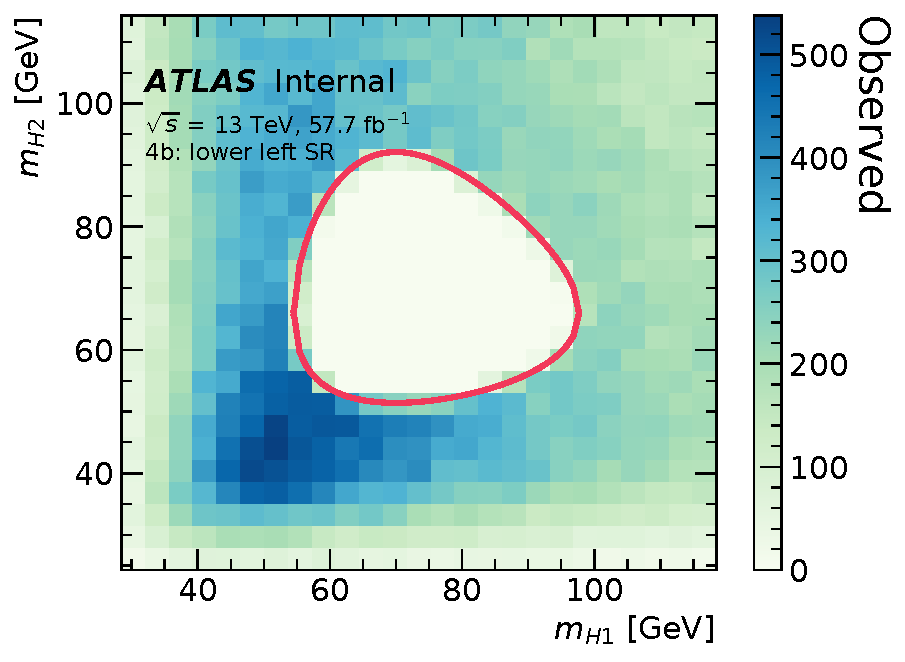
\includegraphics[height=4cm]{\figpath/massplane_obs_18} 
	\label{fig:massplane_obs_18}
	}   
    \subfloat[GP fit]{ 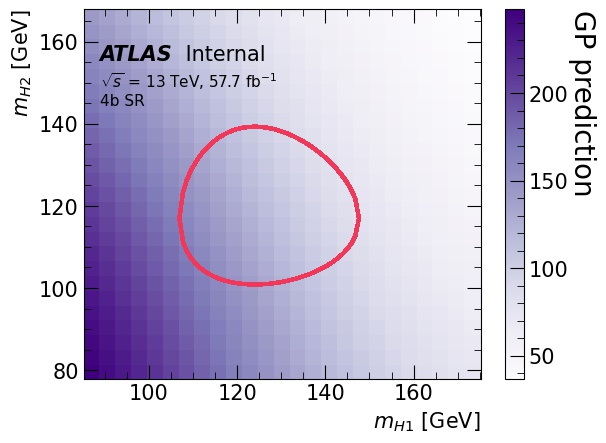
\includegraphics[height=4cm]{
    	\figpath/massplane_pred_18} 
	\label{fig:massplane_pred_18}
	}   
    \subfloat[GP error]{ 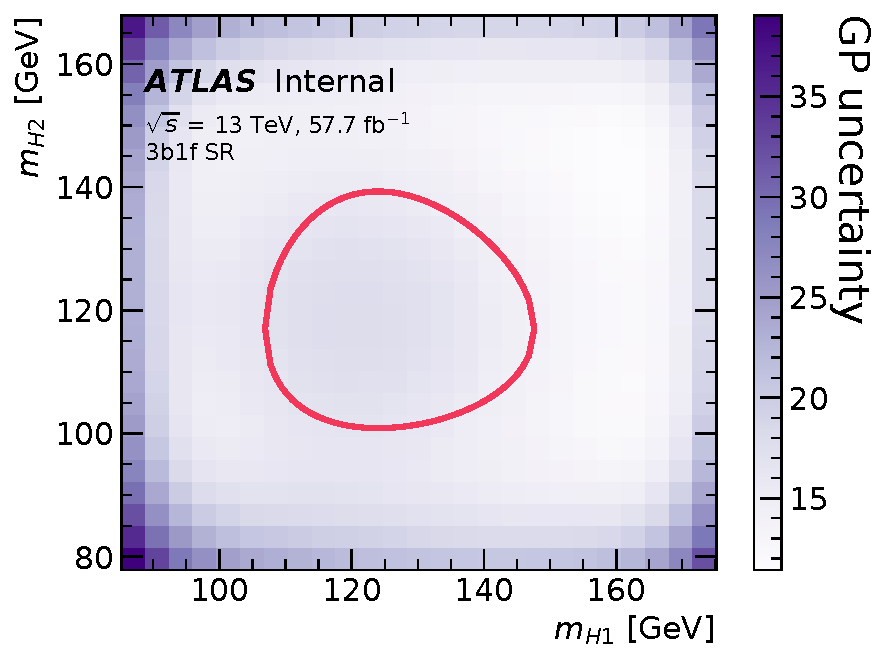
\includegraphics[height=4cm]{
    	\figpath/massplane_prederr_18} 
	\label{fig:massplane_prederr_18}
   	}   
    \caption{GP fits for the 2018 4b \vallabel region. All the massplane fits are before the $X_{Wt}$ cut.}
    \label{fig:gp-\valreg}
\end{figure}	
	
\begin{figure}[ht]
    \centering
    \subfloat[GP closure]{ 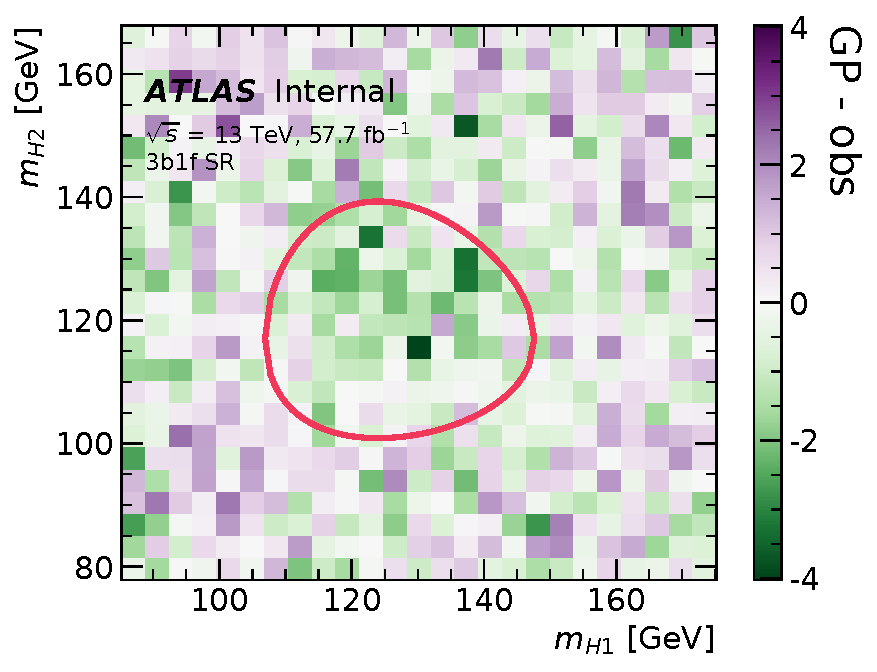
\includegraphics[height=4cm]{
    	\figpath/massplane_pred_minus_obs_over_sqrt_obs_18} 
	\label{fig:massplane_pred_minus_obs_over_sqrt_obs_18}
	}   
    \subfloat[Pulls]{ 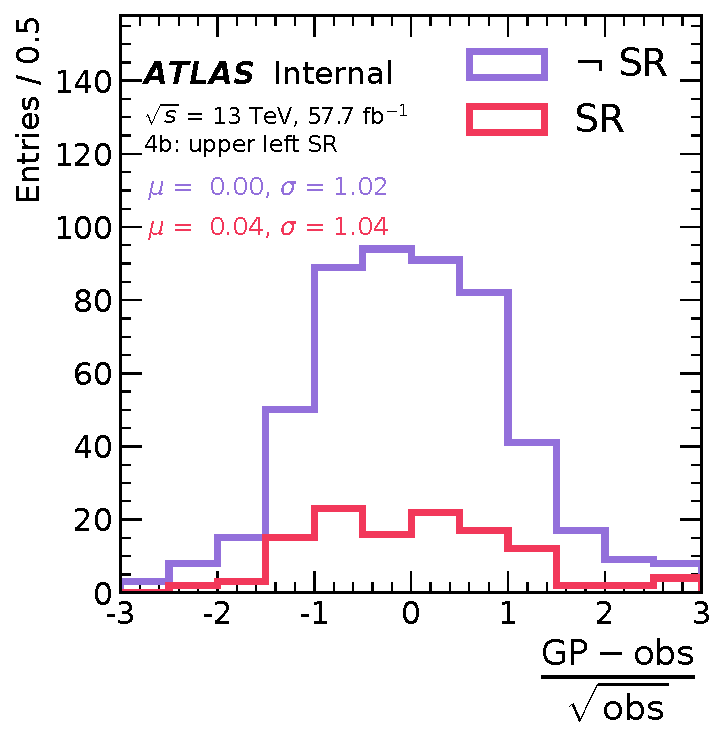
\includegraphics[height=4.5cm]{
    	\figpath/hist_pred_minus_obs_over_sqrt_obs_18} 
	\label{fig:hist_pred_minus_obs_over_sqrt_obs_18}
	}   
    \caption{Left: non-closure of the GP fits for the 2018 4b \vallabel region. 
    Right: 1d histogram of the pulls. The ``$\neg$ SR'' line shows the bins that were included in the GP prediction fit, while the ``SR'' line shows the bins blinded in the fit that had some overlap with the SR.
    The GP fits and these plots are before the $X_{Wt}$ cut.
    }
    \label{fig:gp-\valreg}
\end{figure}

Next we draw samples from this GP to have samples to condition the flow in the SR with.
To find samples from the massplane, we draw samples from the flow using inverse transform sampling.
The samples are taken from the bin centers of the 2d histogram, but then additionally uniformly smeared to take into account the width of the bin.

Finally, since the number of samples that we draw is arbitrary, we rescale the predicted samples templates using the samples from the GP massplane:

\begin{equation}
	n_{SR} = n_{\neg SR}^{obs} \cdot \frac{n_{SR}^{samples}}{n_{\neg SR}^{samples}}.
\end{equation}

%\begin{enumerate}
%\item
%\end{enumerate}

